\begin{mainquestion}{capacitorcurrent}{Capacitor Analysis}

The current $i_C(t)$ through a \qty{200}{\nano\farad} capacitor is shown in the figure below. At $t = 0$, the voltage $v(t)$ is -16 V.

\begin{center}
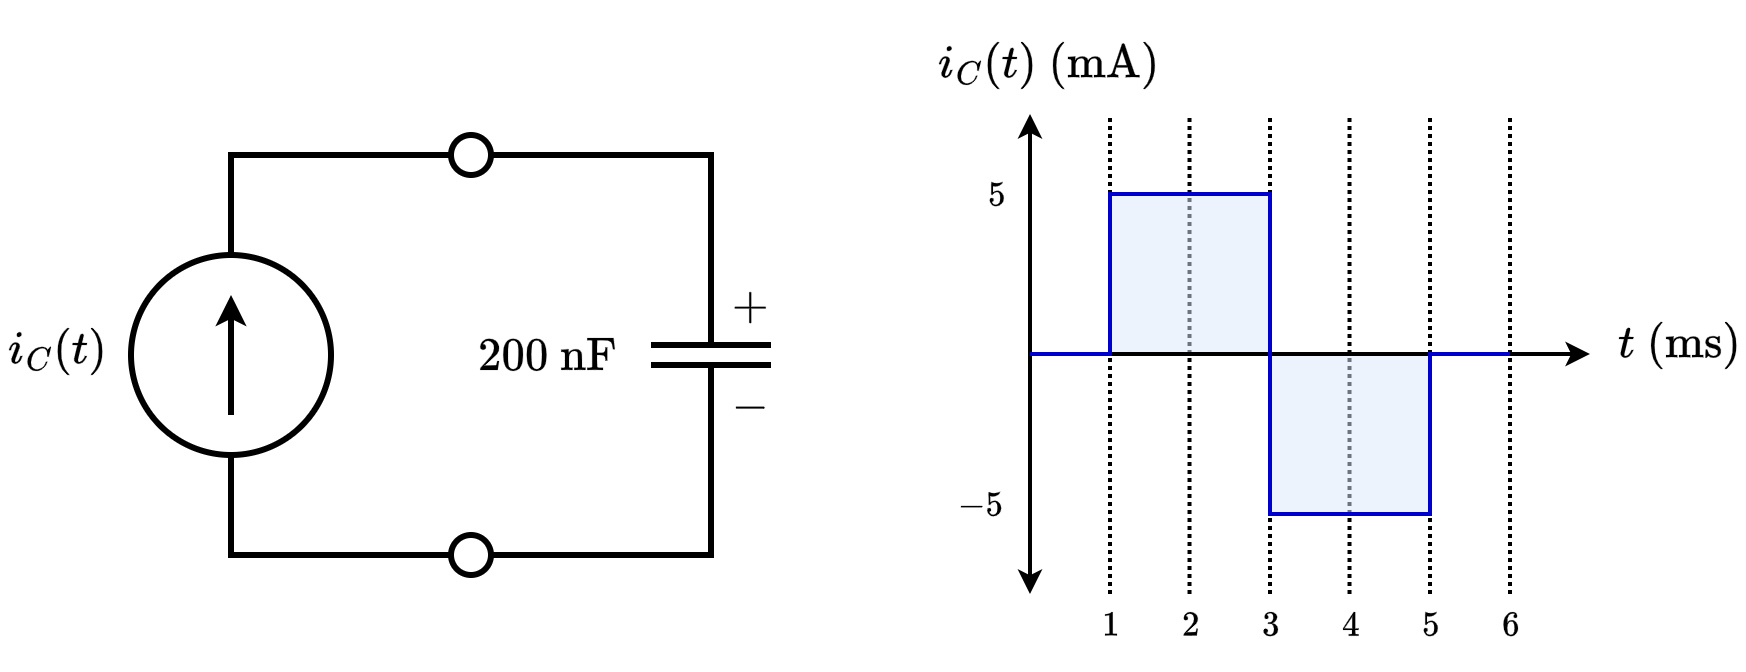
\includegraphics[width=1.0\textwidth]{current_circuit.png}
\end{center}

% =========================================================
\begin{partquestion}{voltagepower}
{Calculate the voltage, power, and stored energy of the capacitor as a function of time.}

\begin{answer}
The equation that relates the current and the voltage in a capacitor is given by:

\[
i_C(t) = C \frac{dv_C(t)}{dt} \quad \Rightarrow \quad v_C(t) = \frac{1}{C}\int i_C(t)\,dt + v_C(0)
\]

Nothing happens until \qty{1}{\milli\second} when the current source begins to output \qty{5}{\milli\ampere}.
From \qty{1}{\milli\second} to \qty{3}{\milli\second}:

\begin{align*}
v_C(t) &= \frac{1}{\num{200e-9}} \int_{0.001}^t \num{5e-3} \,dt' - 16\\
&= \frac{1}{\num{200e-9}} \int_{0}^{t-0.001} \num{5e-3} \,dt' - 16\\
&= (\num{25e3})(t-0.001) - 16 \quad (0.001 \leq t \leq \qty{0.003}{\second}) \\
v_C(0.003) &= 50 - 16 = \qty{34}{\volt}
\end{align*}

From 3 ms to 5 ms the current is reversed, which should cause the voltage to fall back down to where it started.
\begin{align*}
v_C(t) &= \frac{1}{\num{200e-9}} \int_{0.003}^t \num{-5e-3} \,dt' +34\\
&= \frac{1}{\num{200e-9}} \int_{0}^{t-0.003} \num{-5e-3} \,dt' +34\\
&= (\num{-25e3})(t-0.003) +34 \quad (0.003 \leq t \leq \qty{0.005}{\second}) \\
v_C(0.005) &= -50 + 34 = \qty{-16}{\volt}
\end{align*}

Consolidating these results gives:

\[
v_C(t) = \begin{cases}
- 16 & t \leq 0.001 \\
\num{25e3} (t - 0.001) - 16 & 0.001 \leq t \leq 0.003 \\
\num{-25e3} (t - 0.003) + 34 & 0.003 \leq t \leq 0.005 \\
- 16 & t \geq 0.005
\end{cases}
\]

The power stored is given by the product of the current and the voltage in the capacitor, that is, $p_C(t) = v_C(t) \cdot i_C(t)$. Therefore, (measuring power in watts):

\begin{align*}
p_C(t) &= \begin{cases}
(- 16)(0) & t \leq 0.001 \\
(\num{25e3} (t - 0.001) - 16)(0.005) & 0.001 \leq t \leq 0.003 \\
(\num{-25e3} (t - 0.003) + 34)(-0.005) & 0.003 \leq t \leq 0.005 \\
(- 16)(0) & t \geq 0.005
\end{cases} \\
&= \begin{cases}
0 & t \leq 0.001 \\
125(t - 0.001) -0.08 & 0.001 \leq t \leq 0.003 \\
125(t - 0.003) -0.17 & 0.003 \leq t \leq 0.005 \\
0 & t \geq 0.005
\end{cases}
\end{align*}

The energy (measured in joules) stored in the capacitor is given by:

\[
E_C = \frac{1}{2} C V^2 = \frac{1}{2}(\num{200e-9}) v_C(t)^2 = (\num{1e-7}) v_C(t)^2
\]

Using the result for the capacitor voltage from before we can determine:

\begin{align*}
E_C(t) &= \begin{cases}
(\num{1e-7})(-16)^2 & t \leq 0.001 \\
(\num{1e-7})(\num{25e3} (t - 0.001) - 16)^2 & 0.001 \leq t \leq 0.003 \\
(\num{1e-7})(\num{-25e3} (t - 0.003) + 34)^2 & 0.003 \leq t \leq 0.005 \\
(\num{1e-7})(-16)^2 & t \geq 0.005
\end{cases} \\
&= \begin{cases}
\num{25.6e-6} & t \leq 0.001 \\
\num{625e6}t - \num{2.05e6}t + 1681 & 0.001 \leq t \leq 0.003 \\
\num{625e6}t - \num{5.45e6}t + 11881 & 0.003 \leq t \leq 0.005 \\
\num{25.6e-6} & t \geq 0.005
\end{cases}
\end{align*}

\end{answer}
\end{partquestion}

% =========================================================
\begin{partquestion}{waveformplots}
{Plot the current, voltage, power, and stored energy to scale versus time so that the relation between each is clear.}

\begin{answer}
Plotting these graphs gives the results below:

\begin{center}
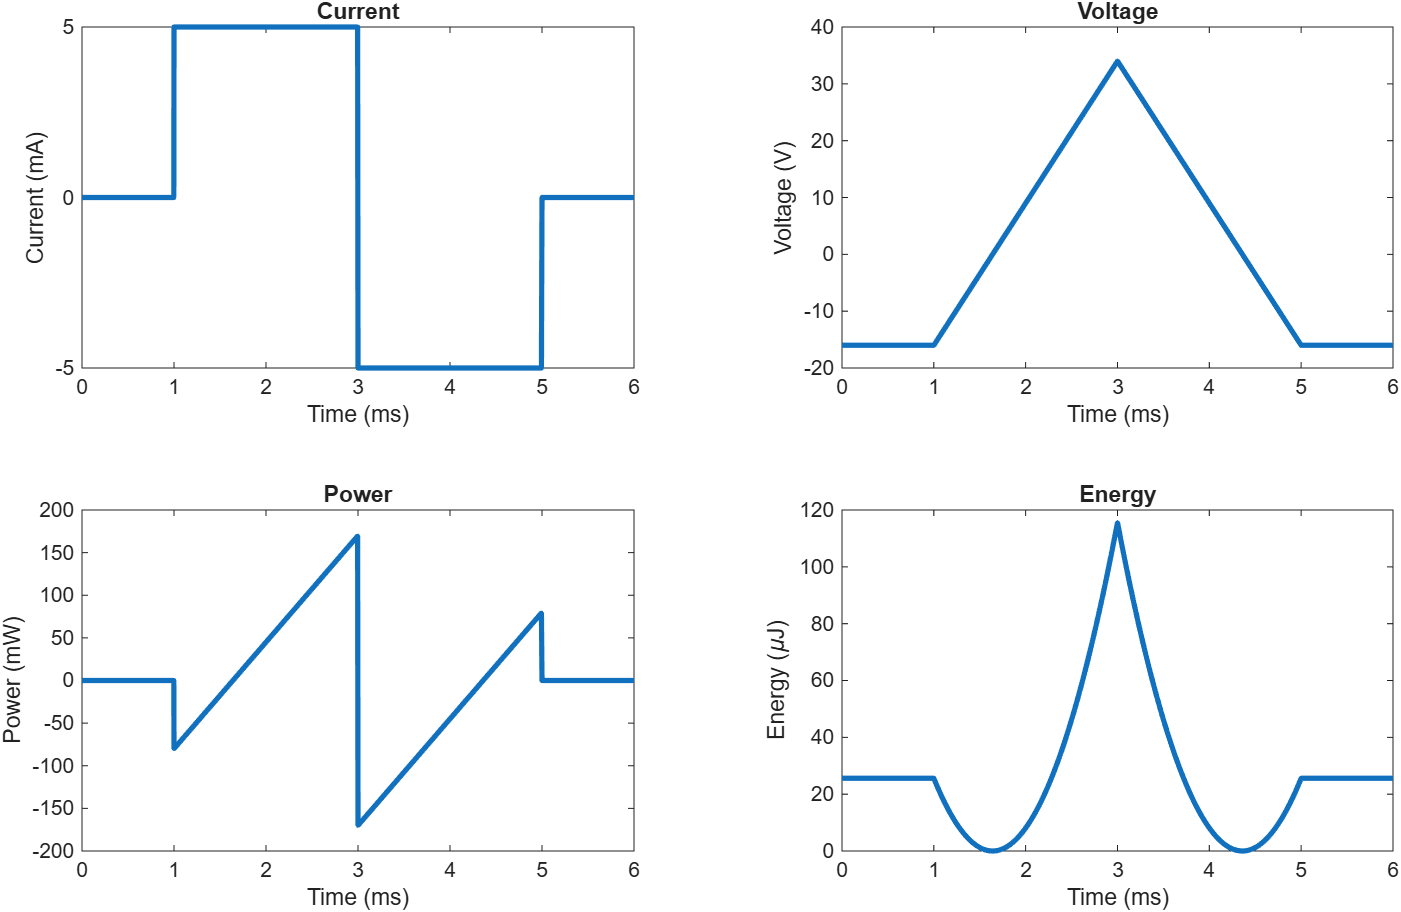
\includegraphics[width=5in]{waveforms.png}
\end{center}

\end{answer}
\end{partquestion}

% =========================================================
\begin{partquestion}{peakpower}
{What is the peak power and at what time $t$ does it occur?}

\begin{answer}
From the graph and our equations it's clear that the peak power (both positive and negative) occurs at \qty{3}{\milli\second} with a value of \qty{170}{\milli\watt}.
\begin{align*}
    p_C(0.003) &= 125(0.003 - 0.001) -0.08 \\
    &= 125(0.002) -0.08 = 0.25 - 0.08\\
    &= \qty{0.170}{\watt}
\end{align*}
\end{answer}
\end{partquestion}

% =========================================================
\begin{partquestion}{zero}
{What is the minimum and maximum energy stored in the capacitor and at which times $t$ do they occur?}

\begin{answer}
The maximum energy will be stored in the capacitor when $|v_C|$ is at its largest, since the energy is computed using the square of voltage. From the graph, it's clear this happens at \qty{3}{\milli\second} when the capacitor has a voltage of \qty{34}{\volt}. We compute the energy as:
\[
E_{C,\text{max}} = \frac{1}{2}CV_C^2 = \frac{1}{2}(\num{2e-7}) (34)^2 = \qty{115.6}{\micro\joule}
\]

The minimum energy is zero! Since the voltage changed from positive to negative during our analysis, sometime in the middle it passed through \qty{0}{\volt}, which would imply $E_C = 0$ at that point. We can solve for that time by either finding the minimum of the energy function, or solving for when the voltage was equal to zero. Here we will solve using the voltage:

\begin{gather*}
\num{25e3} (t_{\text{min,1}} - 0.001) - 16 = 0 \\
t_{\text{min,1}} = \frac{16}{\num{25e3}} + 0.001 \\
t_{\text{min,1}} = 0.00164 = \qty{1.64}{\milli\second}
\end{gather*}

Keep in mind that the energy also drops to zero again when the current reverses from \qty{3}{\milli\second} - \qty{5}{\milli\second}. We can use the other equation to solve for that one:

\begin{gather*}
-\num{25e3} (t_{\text{min,1}} - 0.003) + 34 = 0 \\
t_{\text{min,2}} = \frac{-34}{\num{-25e3}} + 0.003 \\
t_{\text{min,2}} = 0.00436 = \qty{4.36}{\milli\second}
\end{gather*}

\end{answer}
\end{partquestion}


\end{mainquestion}
